\documentclass[main]{subfiles}

\begin{document}


\chapter{Pruebas del controlador}
El controlador diseñado se comporta adecuadamente en lo que respecta a las simulaciones, sin embargo debido a que la caracterizaci\'on del sistema puede contener errores se proceden a realizar algunas pruebas sobre los subsistemas que componen al sistema global. Estas pruebas son de utilidad para verificar el correcto funcionamiento del controlador diseñado y/o para realizar los ajustes que sean necesarios en el mismo.

\section{Control del subsistema del Roll}

Para lograr el correcto funcionamiento del cuadric\'optero es fundamental que el control sobre los \'angulos de Pitch y de Roll se comporte de buena forma. A modo de ejemplo, es imposible lograr el equilibrio mec\'anico si dichos \'angulos difieren de cero. Por dicha raz\'on, previo a realizar pruebas sobre el sistema completo es necesario asegurarnos que los subsistemas del  Roll y del Pitch funcionan correctamente. De acuerdo al modelo f\'isico del sistema desarrollado en \ref{chap:modelo} ni el Roll ni el Pitch son subsistemas independientes entre s\'i, adem\'as ambos dependen de la velocidad angular seg\'un $\vec{k}_q$. Sin embargo, dichos \'angulos toman valores cercanos a cero en las trayectorias de inter\'es, en este caso se puede realizar la aproximaci\'on de que ambos sistemas son independientes.\\

\begin{wrapfigure}{r}{0.55\textwidth}
	\vspace{-20pt}
	\centering
	\includegraphics[width=0.4\textwidth]{./pics_test_control/dispositivo_psi.pdf}
	\caption{Dispositivo de prueba de Roll}
	\label{fig:psidisp}
\end{wrapfigure}

A partir de esta consideraci\'on se procede a fijar al cuadric\'optero sobre dos gu\'ias como se muestra en la figura \ref{fig:psidisp}, de forma de eliminar todos los grados de libertad del sistema excepto el \'angulo de Roll y la velocidad angular correspondiente al eje de rotaci\'on del Roll. Se realizan dos pruebas: la primera consiste en que el sistema alcance la posic\'on de equilibrio ($\psi = 0$), la segunda consiste en alejar al sistema del equilibrio y lograr que vuelva al punto de equilibrio.\\

El controlador posee dos terminos proporcionales: uno para el \'angulo $\psi$ y el otro para la velocidad angular $\omega_{qx}$ y un t\'ermino integral asociado a la integral de $\psi$. El modelo de este subsistema es el siguiente: 

\begin{equation}
\left(\begin{array}{c}
\dot{\psi}\\
\dot{\omega}_{qx}\\
\dot{\psi_I}
\end{array}\right) = \left(\begin{array}{ccc}
0 & 1 & 0\\
-\frac{MgL^\prime}{I_{xx}} & 0 & 0\\
1 & 0 &1
\end{array}\right) + b\left(\begin{array}{cc}
0 & 0\\
1 & -1\\
0 & 0\\
\end{array}\right) \left(\begin{array}{c}
\omega_2 \\
\omega_4
\end{array}\right)
\end{equation}

Donde $b$ y $\frac{MgL^\prime}{I_{xx}}$ son los obtenidos en la secci\'on \ref{chap:verificaciones}. La matriz de realimentaci\'on obtenida trabajando con las matrices $Q$ y $R$ definidas en \ref{eq:Q_R_roll} es:

\begin{equation}
\label{K_roll}
K = \left( \begin{array}{ccc}
44.43 & 10.78 &21.36\\
-44.430 & -10.78 &-21.36
\end{array}\right)
\end{equation}
\begin{equation}
\label{eq:Q_R_roll}
Q = \left(\begin{array}{ccc}
1000 & 0 & 0\\
0 & 1 & 0\\
0 & 0 & 100 
\end{array} \right) \quad R =\left(\begin{array}{cc}
0.1 & 0 \\
0 & 0.1
\end{array}\right)
\end{equation}\\	


\begin{wrapfigure}{r}{0.55\textwidth}
	\vspace{-20pt}
	\centering
	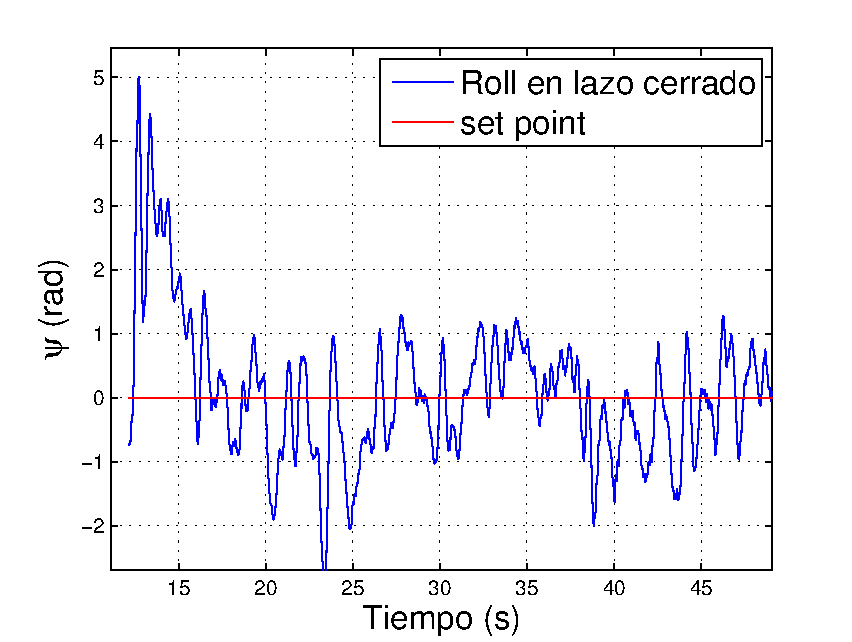
\includegraphics[width=0.4\textwidth]{./pics_test_control/psi.pdf}
	\caption{\'Angulo de Roll en lazo cerrado}
	\label{fig:psi}
\end{wrapfigure}

En la figura \ref{fig:psi} se observa la respuesta del \'angulo de Roll en lazo cerrado. Con el setpoint fijo en $\psi = 0$ se observa que el m\'odulo del \'angulo es siempre inferior a los $2^\circ$ a excepci\'on del arranque y en un pico cerca de los 23 segundos. En este sentido se puede afirmar que el control implementado es exitoso, ya que logra el objetivo planteado. Puede observarse adem\'as que una vez que el controlador comienza a actuar se produce un cambio en el \'angulo alcanzando un valor cercano a los $5 ^\circ$. Este error es producido por la diferencia del empuje de los motores frente a una misma orden. El control integral es el encargado de corregir esta diferencia en aproximadamente $2.5$ segundos, un tiempo que es considerado aceptable.\\

\begin{wrapfigure}{l}{0.55\textwidth}
	\vspace{-20pt}
	\centering
	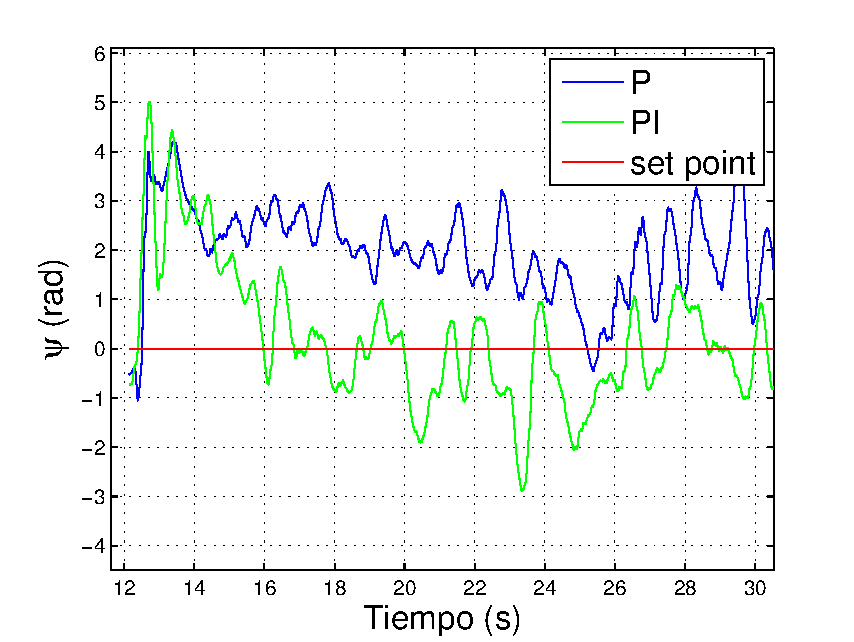
\includegraphics[width=0.4\textwidth]{./pics_test_control/psi_sin_con_int.pdf}
	\caption{\'Angulo de Roll en lazo cerrado}
	\label{fig:psi_sin_con_int}
\end{wrapfigure}

En la figura \ref{fig:psi_sin_con_int} se puede observar la diferencia entre utilizar un controlador puramente proporcional y un controlador proporcional con una correcci\'on integral. El primero no logra corregir el error sistem\'atico debido a la diferencia en el empuje de los motores alcanzando as\'i un punto de equilibrio distinto del \emph{set point}. El controlador con el t\'ermino integral si logra corregir este error y el \'angulo $\psi$ toma valores en el entorno del \emph{set point}.\\


\begin{wrapfigure}{r}{0.50\textwidth}
	\vspace{10pt}
	\centering
	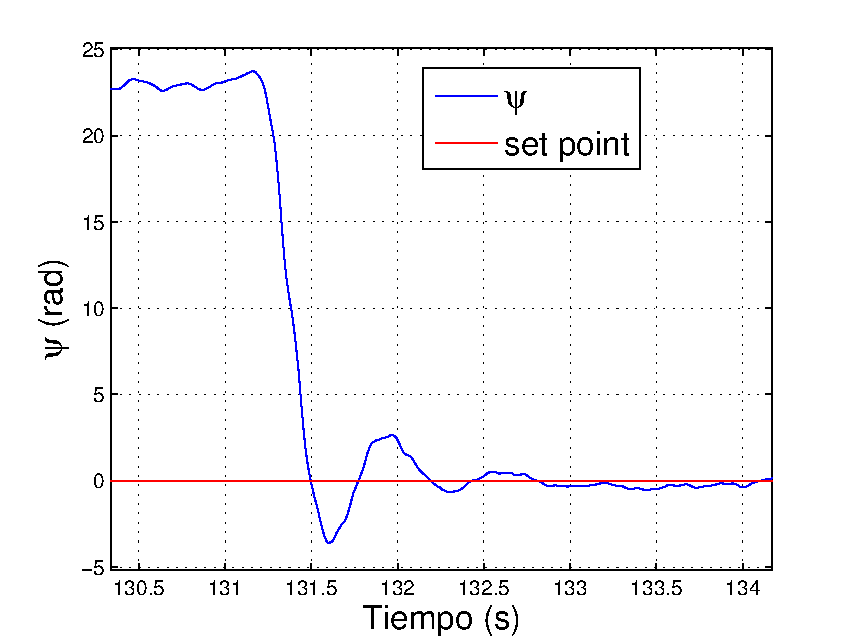
\includegraphics[width=0.4\textwidth]{./pics_test_control/psi_esc.pdf}
	\caption{Respuesta al escal\'on del \'angulo de Roll en lazo cerrado}
	\label{fig:psi_esc}
\end{wrapfigure}

Resulta fundamental entender como es la respuesta del sistema realimentado para apartamientos considerables respecto del equilibrio. Dicha situaci\'on puede producirse por diversas razones, un leve golpe de alg\'un agente externo o una simple turbulencia. En la figura \ref{fig:psi_esc} puede observarse la respuesta al escal\'on del sistema en lazo cerrado	con \'angulo inicial de aproximadamente $23 ^\circ$ y \emph{set point} $0 ^\circ$. La respuesta del sistema es muy buena, ya que se logra el valor de \emph{set point} en aproximadamente un segundo y la misma presenta un sobretiro del orden del $10\%$. \\

Con este an\'alisis se concluye que la matriz de realimentaci\'on obtenida es adecuada para controlar el subsistema del \'angulo de Roll. El comportamiento del \'angulo de Pitch es similar al de Roll y por dicho motivo no ser\'a presentado. 

\section{Control del subsistema del Yaw}


De manera an\'aloga al caso anterior, es importante verificar el buen funcionamiento del control sobre el giro en ``z'', para lo cual se utiliza un dispositivo de prueba que restringe los grados de libertad del cuadric\'optero. En este caso se lo sujeta con una cuerda desde arriba de los cuatro brazos de modo de realizar la fuerza lo m\'as pareja posible. El cuadric\'optero queda sujetado colgando horizontal y conserva el libre giro seg\'un ``z'' ($\theta$).
Se setea una velocidad de \emph{hovering} inferior a la necesaria para levantar vuelo, de modo que el cuadric\'optero no se eleve y la cuerda quede siempre tensa. Para el giro bajo estudio no es relevante el valor absoluto de la velocidad de giro de cada motor, ya que depende exclusivamente de la diferencia de velocidades angulares. Por ello los resultados de realizar las pruebas con una velocidad de \emph{hovering} inferior a la real son extrapolables a la situaci\'on de vuelo libre, sin p\'erdida de generalidad.\\

\begin{wrapfigure}{r}{0.55\textwidth}
	\vspace{-20pt}
	\centering
	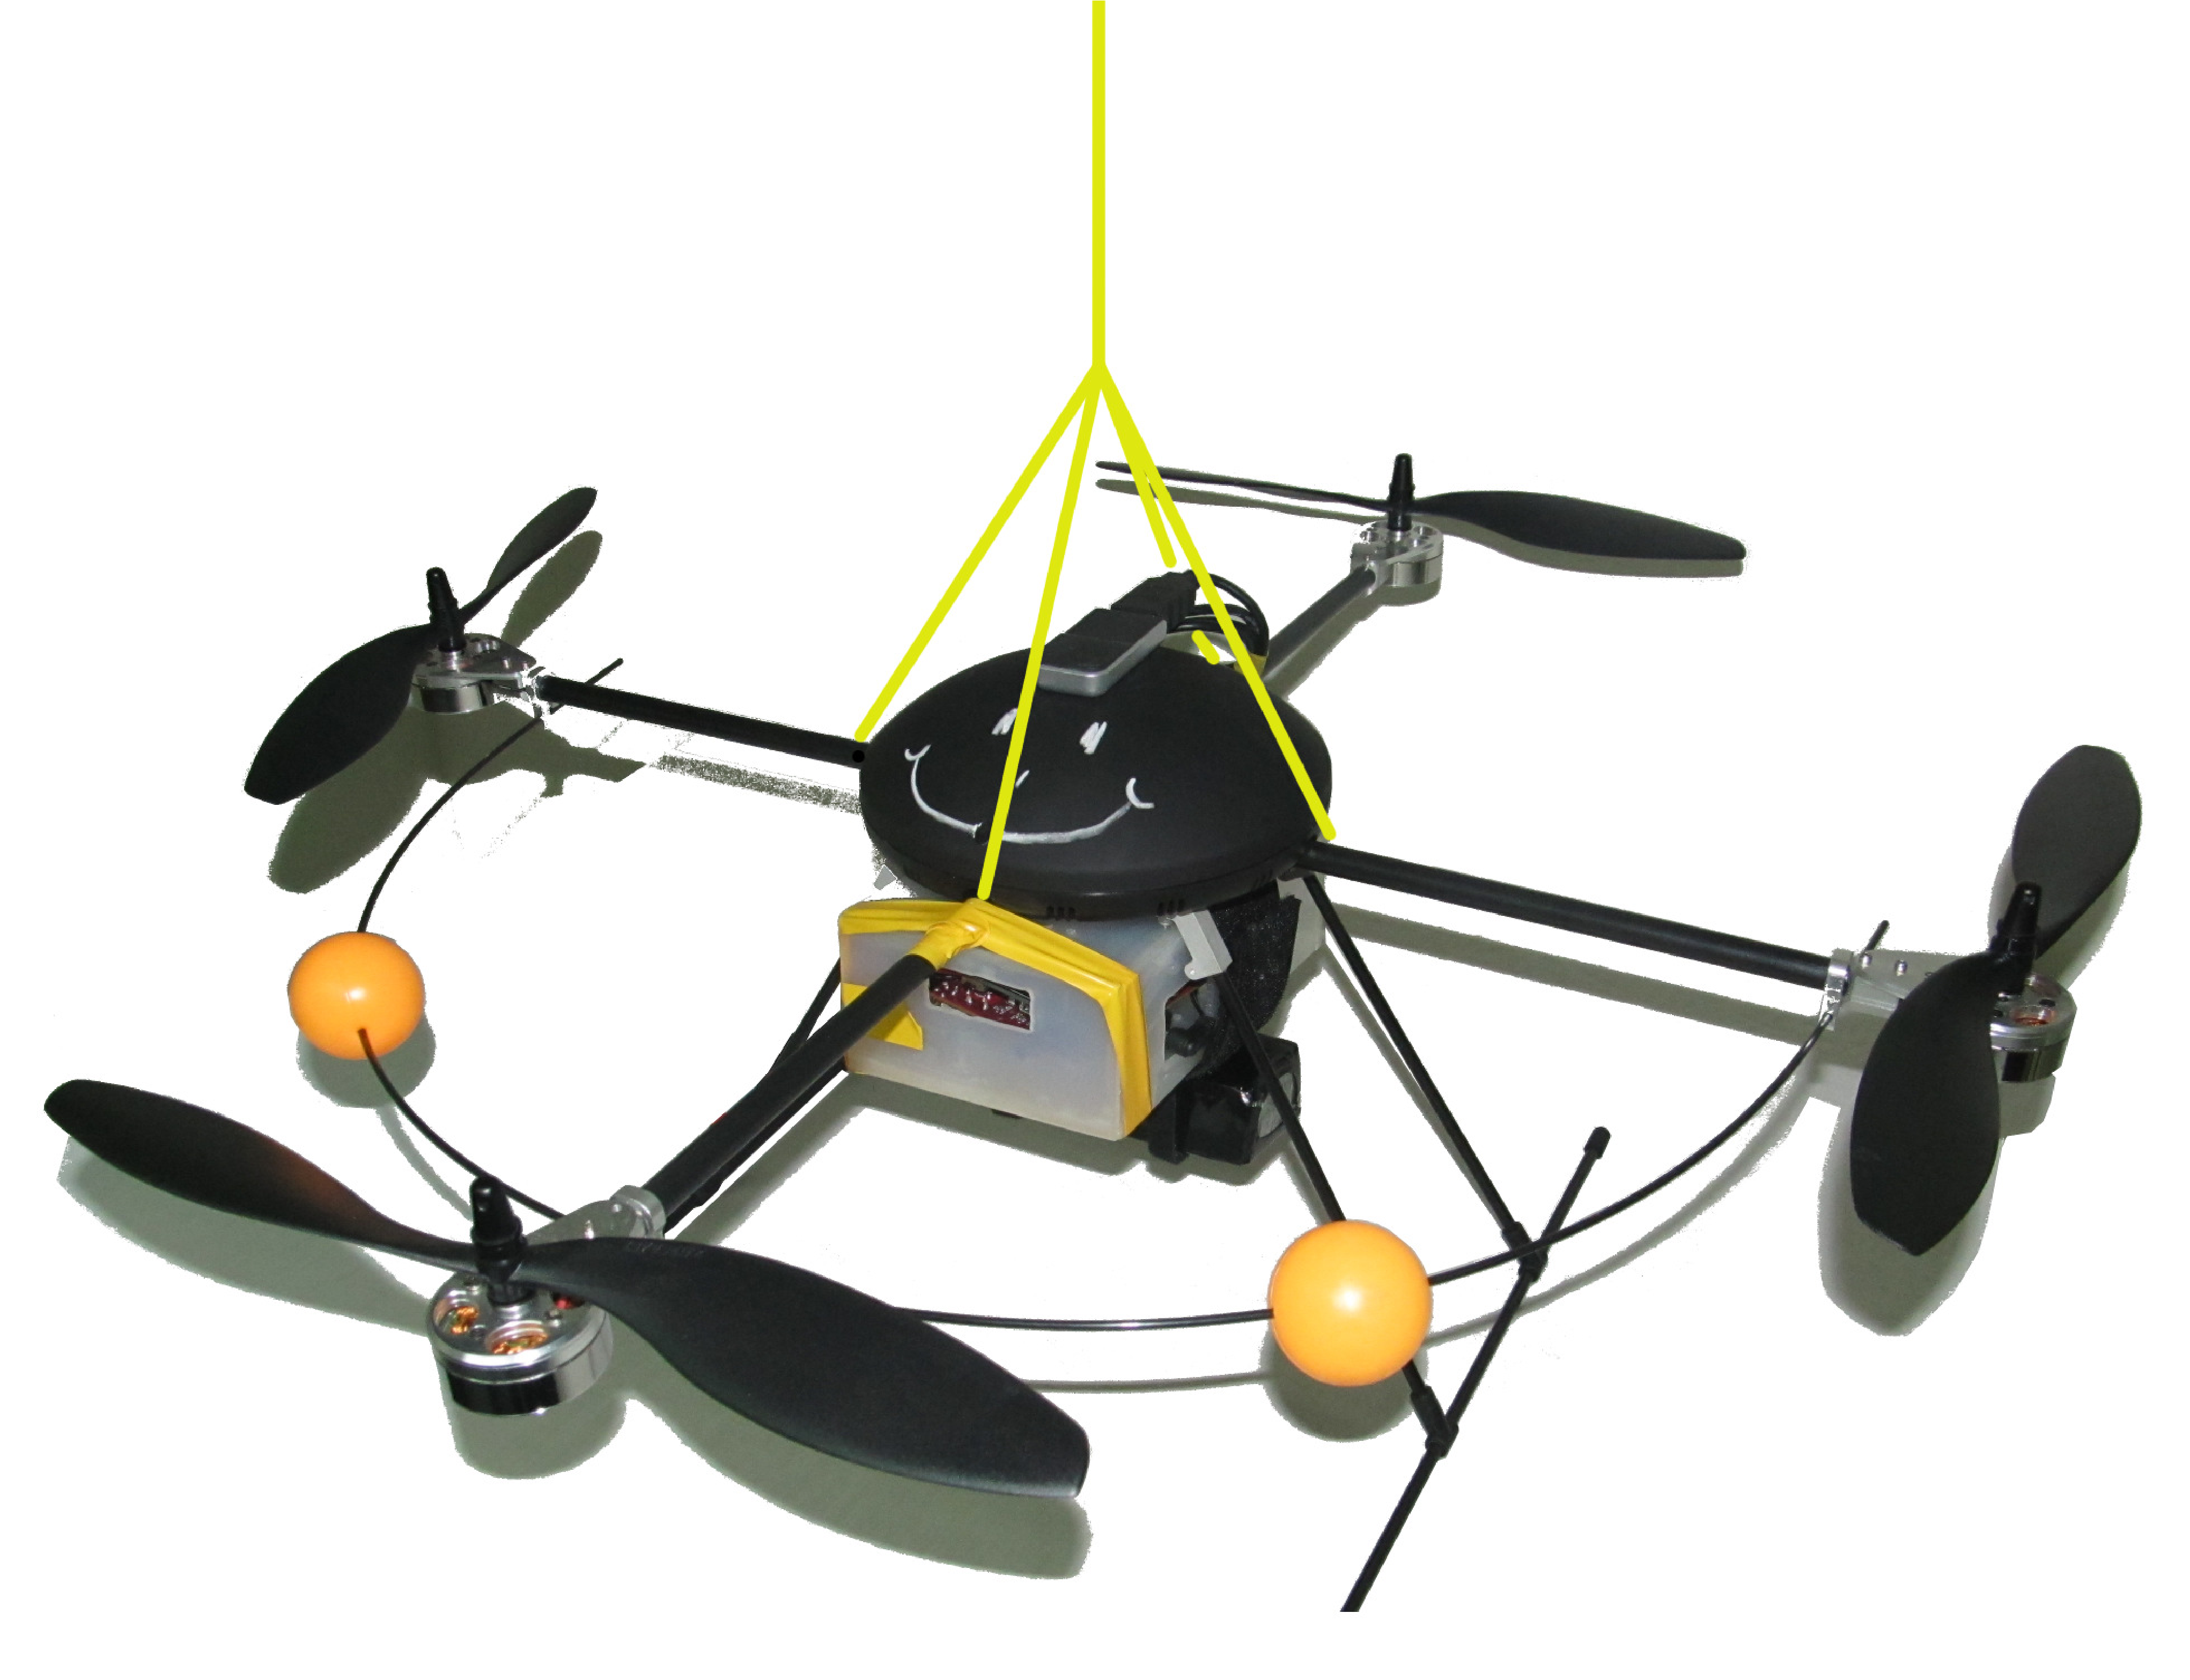
\includegraphics[width=0.4\textwidth]{./pics_test_control/dispositivo_theta.pdf}
	\caption{Dispositivo de prueba de $\theta$}
	\label{fig:thetadisp}
\end{wrapfigure}

El giro en $\theta$ es generado por un desequilibrio entre los pares ejercidos por las h\'elices. Si el par neto de todas las h\'elices resulta por ejemplo positivo, el cuadric\'optero realizar\'a un movimiento hacia los negativos, equilibrando el par, como se explica en el cap\'itulo \ref{chap:general}.\\

Para la estimaci\'on de $\theta$ se utiliza por un lado la integral de la velocidad angular en el eje ``z'' y por otro la proyecci\'on del vector del campo magn\'etico medido sobre el plano horizontal, medidas que son combinadas en el filtro de Kalman. El dato obtenido del magnet\'ometro no distingue entre giros de $360^o$, limitando el valor al rango [$-180^o$ - $180^o$]. Es necesario entonces realizar un reajuste de la medida deducida del campo magn\'etico para lograr la continuidad en el \'angulo estimado.\\

\end{document}